%   Filename    : chapter_4.tex 
\chapter{Results and Discussion/System Prototype}
\section{Data Gathering}
The data for dengue case prediction was gathered from a variety of reliable sources, enabling a comprehensive dataset spanning from January 2011 to October 2024. This dataset includes 720 rows of data, each containing weekly records of dengue cases along with corresponding meteorological variables, such as rainfall, temperature, and humidity.
\begin{enumerate}
	\item Dengue Case Data: The primary source of historical dengue cases came from the Humanitarian Data Exchange and the Western Visayas Center for Health Development (WVCHD). The dataset, accessed through Freedom of Information (FOI) requests, provided robust case numbers for the Western Visayas region. The systematic collection of these data points was essential for establishing a reliable baseline for model training and evaluation.
	\item Weather Data: Weekly weather data was obtained by web scraping from Weather Underground, allowing access to rainfall, temperature, wind, and humidity levels that correlate with dengue prevalence.
\end{enumerate}

\begin{figure}[ht]
	\centering
	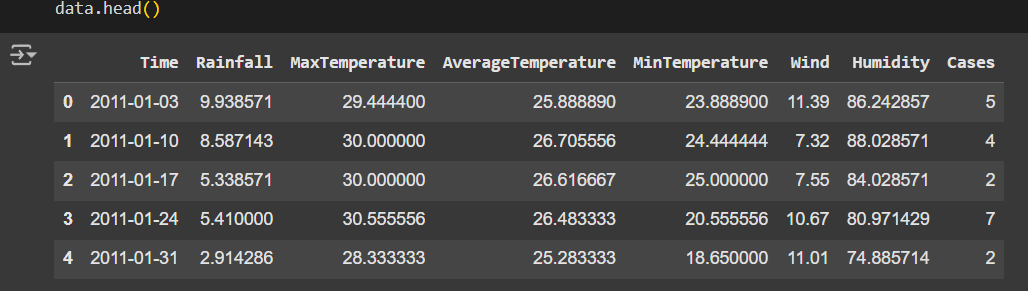
\includegraphics[width=0.95\textwidth]{data_snippet}
	\caption{Snippet of the Combined Dataset}
	\label{fig:data_snippet}
\end{figure}

\section{Exploratory Data Analysis}

\begin{figure}[h!]
	\centering
	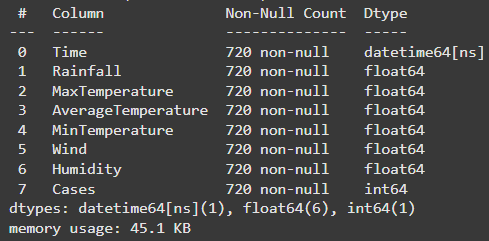
\includegraphics[width=0.75\textwidth]{data_summary}
	\caption{Data Contents}
	\label{fig:data_summary}
\end{figure}

From the summary above, the dataset consists of 720 weekly records with 8 columns:
\begin{itemize}
	\item \textbf{Time.} Weekly timestamps (e.g. "2011-w1")
	\item \textbf{Rainfall.} Weekly average rainfall (mm)
	\item \textbf{MaxTemperature, AverageTemperature, MinTemperature.} Weekly temperature data (C)
	\item \textbf{Wind.} Wind speed (m/s)
	\item \textbf{Humidity.} Weekly average humidity (\%)
	\item \textbf{Cases.} Reported dengue cases
\end{itemize}

\begin{figure}[h!]
	\centering
	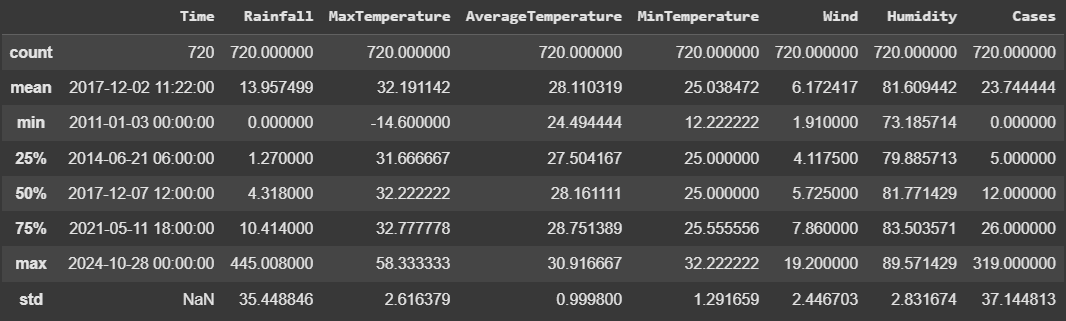
\includegraphics[width=1\textwidth]{data_stats2}
	\caption{Dataset Statistics}
	\label{fig:data_stats2}
\end{figure}

From the statistics in figure \ref{fig:data_stats2}, the number of cases ranges from 0 to 319. The average number of dengue cases per week is 23.74, with a median of 12 cases and a standard deviation of 37.14. The distribution is highly skewed, with some weeks experiencing significant number of cases (up to 319 cases). Rainfall shows a wide variation (0 to 445mm), while temperature remains relatively stable, with an average of 28.1 degree celsius. Humidity levels ranges from 73\% to 89\% with a mean of 81.6\%.

\begin{figure}[ht]
	\centering
	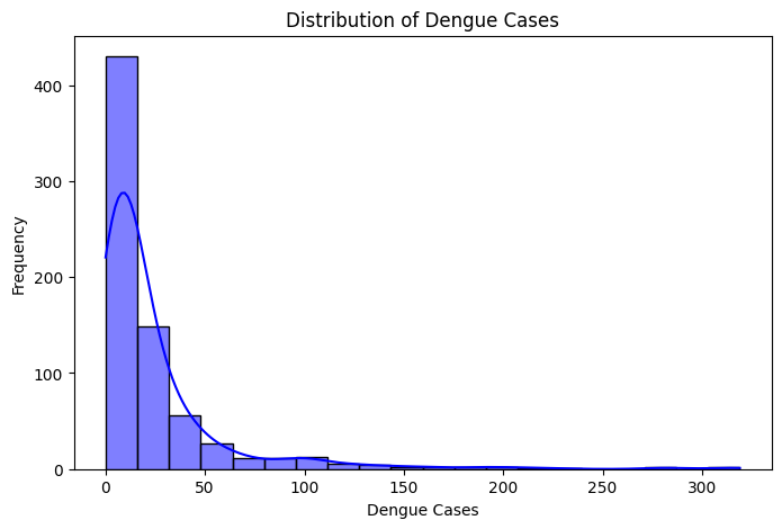
\includegraphics[width=0.75\textwidth]{data_stats}
	\caption{Distribution of Dengue Cases}
	\label{fig:data_stats}
\end{figure}

In figure \ref{fig:data_stats}, a histogram of dengue cases shows a right-skewed distribution, indicating that most weeks experience low case counts, while a few weeks record outbreaks. 
\\To further analyze the distribution, dengue cases were categorized into different intervals (Figure \ref{fig:dengue_intervals}): 0-5 cases, 6-15 cases, 16-30 cases, 31-100 cases and 101+ cases. The majority of weeks falls within the 0-5 cases and 6-15 cases categories, indicating that most weeks have low dengue cases. Meanwhile, weeks with 101+ cases are rare, suggesting that extreme outbreaks are not frequent.
\begin{figure}[ht]
	\centering
	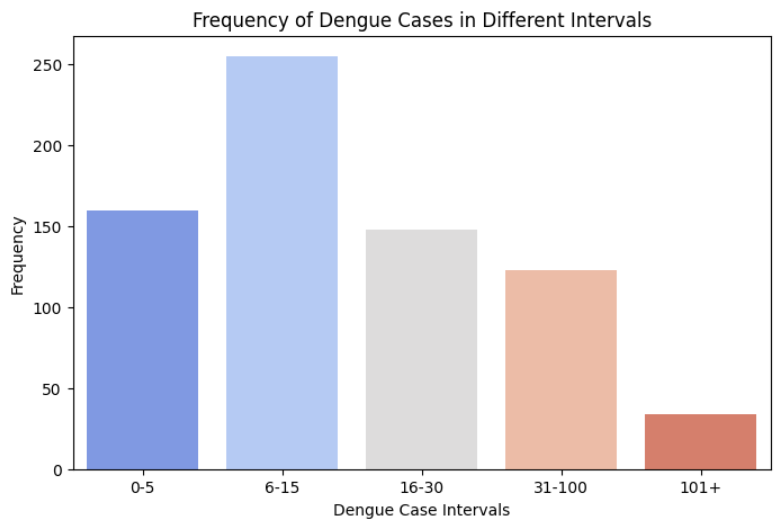
\includegraphics[width=0.75\textwidth]{dengue_intervals}
	\caption{Frequency of Dengue Cases in Different Intervals}
	\label{fig:dengue_intervals}
\end{figure}

Figure \ref{fig:data_trend} illustrates the trend of weekly dengue cases over time. The data reveals periodic spikes in the number of cases, suggesting a seasonal pattern in dengue cases. Notably, peak cases are observed during certain periods approximately 3 years, potentially aligning with specific climatic conditions such as increased rainfall or temperature changes. This underscores the importance of incorporating climate variables into the forecasting model.

\begin{figure}[ht]
	\centering
	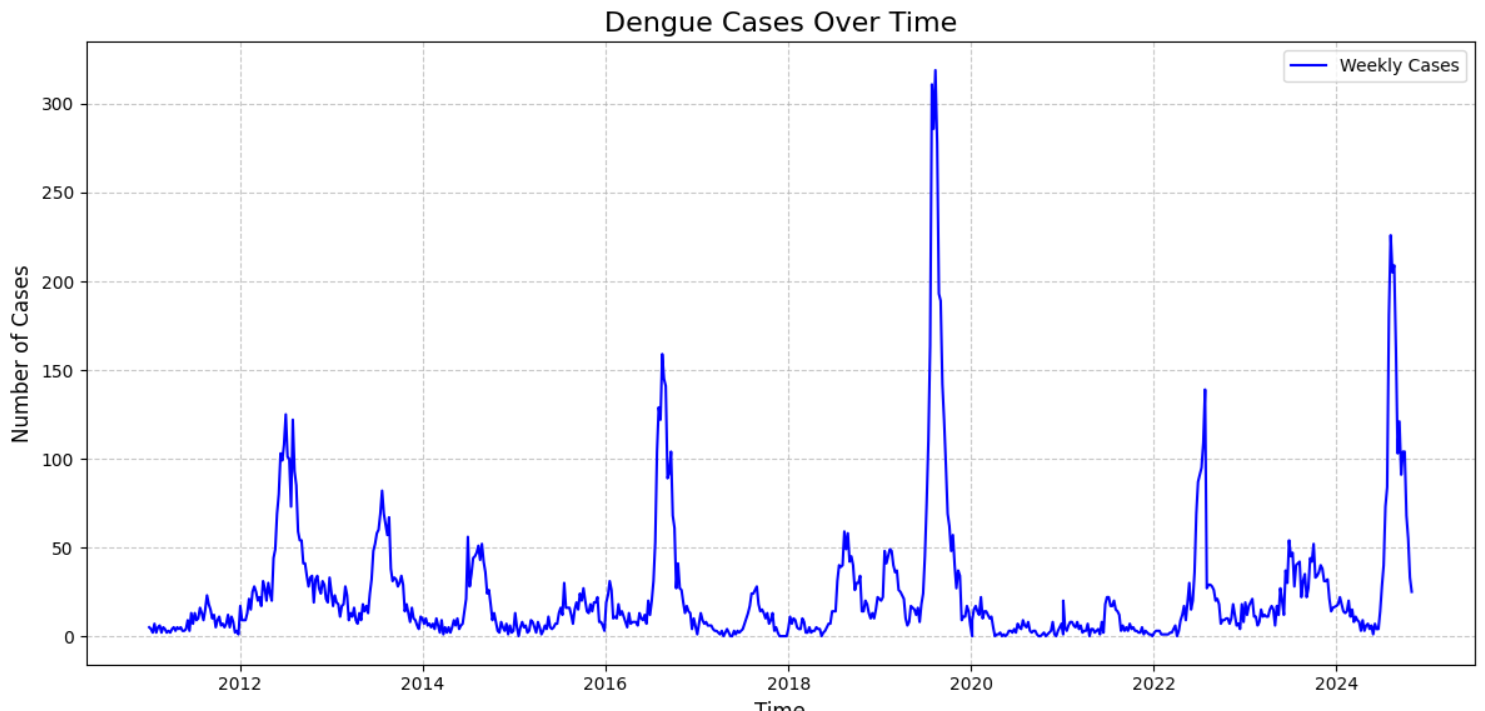
\includegraphics[width=0.90\textwidth]{dengue_trend}
	\caption{Trend of Dengue Cases}
	\label{fig:data_trend}
\end{figure}

Figure \ref{fig:correlation_bar} shows the ranking of correlation coefficients between dengue cases and selected features, including rainfall, humidity, maximum temperature, average temperature, minimum temperature, and wind speed. Among these, rainfall exhibits the highest positive correlation with dengue cases (correlation coefficient ~0.13), indicating that increased rainfall may contribute to higher cases counts. This aligns with existing studies suggesting that stagnant water from heavy rainfall creates breeding grounds for mosquitos. It is followed by humidity (~0.10), suggesting that higher humidity levels may enhance mosquito reproduction, leading to more dengue cases. Temperature has a weak to moderate positive correlation with dengue cases, with maximum temperature (0.09) showing a stronger relationship than average and minimum temperature. 

\begin{figure}[hbt!]
	\centering
	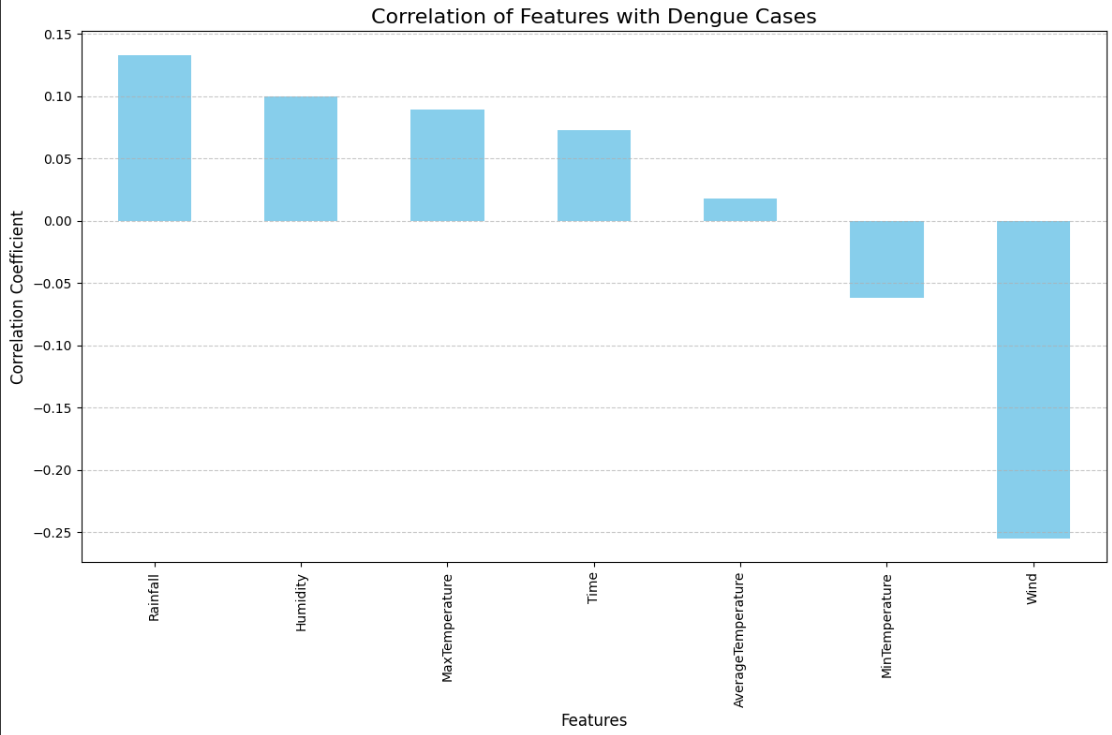
\includegraphics[width=0.75\textwidth]{correlation_bar}
	\caption{Ranking of Correlations}
	\label{fig:correlation_bar}
\end{figure}

Figure \ref{fig:lagged_correlation_bar} shows the ranking of correlation coefficients between dengue cases and selected features, with the addition of lagged effects. The analysis reveals no improvement in correlation when lagged variables are compared to direct observations. This suggests that the observed values of rainfall, humidity, and maximum temperature remain the most significant predictors for dengue case forecasting. Overall, the exploratory data analysis highlights the significance of rainfall, humidity, and max temperature variables in dengue case forecasting.

\begin{figure}[h!]
	\centering
	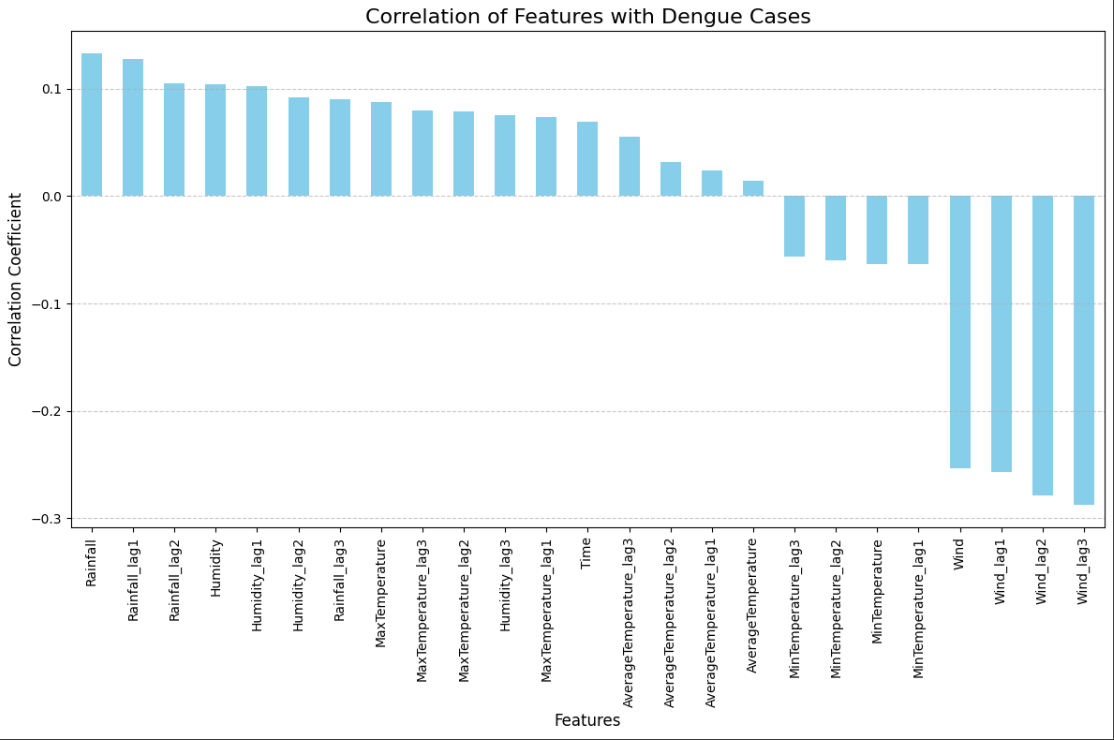
\includegraphics[width=0.75\textwidth]{lagged_correlation_bar}
	\caption{Ranking of Correlations (with lagged effects)}
	\label{fig:lagged_correlation_bar}
\end{figure}

\section{Outbreak Detection}  
To identify outbreaks, we calculated the outbreak threshold value using the historical mean as the endemic channel. The threshold is determined using the formula:  

\begin{align}  
	\text{Outbreak Threshold Value} &= \mu + 2\sigma \\  
	&= 23.744444 + 2(37.144813) \\  
	&= 23.744444 + 74.289626 \\  
	&= 98.03407  
\end{align}  

where \(\mu\) is the historical mean and \(\sigma \) is the standard deviation.

This result indicates that dengue cases exceeding 98 in Iloilo City can be considered an outbreak. However, it is important to note that this threshold serves only as a baseline. Additional parameters, such as the number of hospital beds available in the city, must be considered to compute a more effective threshold and develop an appropriate response strategy.

	
\section{Model Training Results}

The models were evaluated using three metrics: MSE, RMSE, and MAE. The table below provides a summary and comparative analysis of each model’s results across these metrics, offering insights into the strengths and limitations of each forecasting technique for dengue case prediction in Iloilo City. The lower values of the three metrics indicate better forecasting performance. Table \ref{tab:comparison_of_models} shows that the models performed differently on testing data. LSTM outperformed the other models with the lowest RMSE, MSE, and MAE while the other three models had relatively higher values for the three metrics.

\begin{table}[h!]
	\centering
	\resizebox{1\textwidth}{!}{%
		\begin{tabular}{|l|c|c|c|c|c|}
			\hline
			\textbf{Method} & \textbf{LSTM} & \textbf{Seasonal ARIMA} & \textbf{ARIMA} & \textbf{Kalman Filter} & \textbf{KF-LSTM} \\ 
			\hline
			\textbf{Testing MSE}   & 285.54 & 1261.20 & 1521.48 & 1474.82 & 785.35 \\ 
			\hline
			\textbf{Testing RMSE}  & 16.90  & 34.45  & 39.00 & 38.40 & 25.56 \\ 
			\hline
			\textbf{Testing MAE}   & 9.45  & 18.73  & 25.80 & 22.33 & 14.55 \\ 
			\hline
			\textbf{Best Parameters}   
			& \begin{tabular}[c]{@{}c@{}}Window Size: 5\\ Learning Rate: 0.01\\ Units: 64\end{tabular}  
			& (2,0,2)(0,1,1)  
			& (1,2,2) 
			& \begin{tabular}[c]{@{}c@{}}Observation Covariance: 10.0\\ Transition Covariance: 0.1 $\times$ Identity\end{tabular}
			& Same as LSTM \\ 
			\hline
		\end{tabular}%
	}
	\caption{Comparison of different models for dengue prediction}
	\label{tab:comparison_of_models}
\end{table}




\subsection{LSTM Model}
The LSTM model was tuned for the following parameters: learning rate and units. The hyperparameter tuning was conducted for each window size, finding the best parameters for each window size. Further evaluating which window size is most suitable for the prediction model, Table \ref{tab:comparison_of_lstm} shows the evaluation metrics for each window size used in the LSTM model training.
\begin{table}[h!]
	\centering
	\begin{tabular}{|l|c|c|c|c|}
		\hline
		\textbf{Window Size} & \textbf{MSE} & \textbf{RMSE} & \textbf{MAE} & \textbf{R²}\\ \hline
		\textbf{5} & \textbf{285.54} & \textbf{16.90} & \textbf{9.45} & \textbf{0.83}\\ \hline
		\textbf{10} & \textbf{334.63} & \textbf{18.29} & \textbf{9.85} & \textbf{0.80}\\ \hline
		\textbf{20} & \textbf{294.85} & \textbf{17.17} & \textbf{9.35} & \textbf{0.83}\\ \hline
	\end{tabular}
	\caption{Comparison of Window Sizes}
	\label{tab:comparison_of_lstm}
\end{table}

The results indicate that a window size of 5 weeks provides the most accurate predictions, as evidenced by the lowest MSE and RMSE values. Furthermore, the R² score of 0.83 indicates that 83\% of the variability in the target variable (cases) is explained by the independent variables (the inputs) in the model, making it a reliable configuration overall.

Figure \ref{fig:tcsv_training} illustrates the model’s performance in predicting dengue cases for each fold using a window size of 5. As shown in the plot, the training set progressively increases with each fold, mimicking a real-world scenario where more data becomes available over time for dengue prediction. Figure \ref{fig:tcsv_testing} demonstrates that the predicted cases closely follow the trend of the actual cases, indicating that the LSTM model successfully captures the underlying patterns in the data. It is also evident that as the fold number increases and the training set grows, the accuracy of the predictions on the test set improves. Despite the test data being unseen, the model exhibits a strong ability to generalize, suggesting it effectively leverages past observations to predict future trends.

\begin{figure}[H]
	\centering
	\includegraphics[width=1\textwidth]{TSCV_training}
	\caption{Training Folds - Window Size 5}
	\label{fig:tcsv_training}
\end{figure}

\begin{figure}[H]
	\centering
	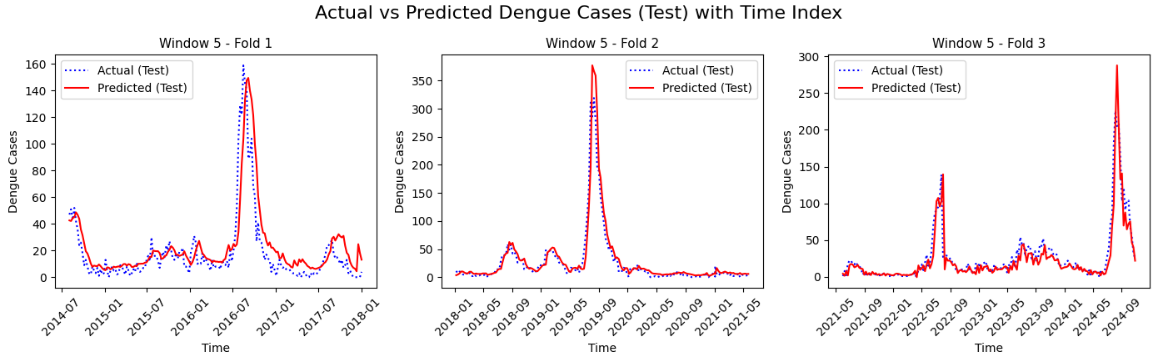
\includegraphics[width=1\textwidth]{TCSV_testing}
	\caption{Testing Folds - Window Size 5}
	\label{fig:tcsv_testing}
\end{figure}

\subsection{ARIMA Model}



\begin{figure}[H]
	\centering
	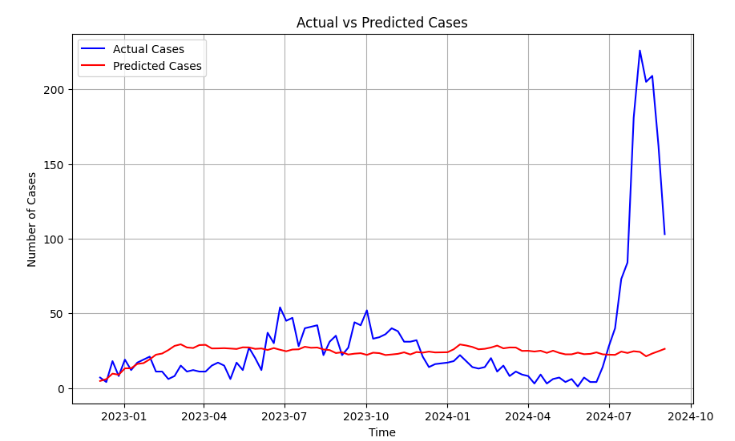
\includegraphics[width=1\textwidth]{line_graph_Arima}
	\caption{ARIMA Prediction Results for Test Set}
	\label{fig:Arima_result}
\end{figure}

The ARIMA model was developed to capture non-seasonal trends in the data. To determine the best model configuration, grid search was used to explore various combinations of ARIMA parameters, ultimately selecting \textbf{ARIMA(1, 2, 2)}. The model was iteratively refined over \textbf{400 iterations} to ensure convergence to an optimal solution. Figure \ref{fig:Arima_result} illustrates the comparison between actual and predicted dengue cases in the test set. As shown in the plot, the ARIMA model struggled to capture the non-linear characteristics and abrupt spikes in the data. Consequently, it failed to accurately reflect the fluctuations and outbreak patterns seen in the actual case counts.

The model's performance was assessed using regression metrics to evaluate its forecasting capability. The ARIMA model yielded the following error metrics:

\begin{itemize}
	\item \textbf{MSE (Mean Squared Error)}: 1521.48
	\item \textbf{RMSE (Root Mean Squared Error)}: 39.01
	\item \textbf{MAE (Mean Absolute Error)}: 25.80
\end{itemize}

\subsection{Seasonal ARIMA (SARIMA) Model}

To address the limitations of the ARIMA model, a Seasonal ARIMA (SARIMA) model was developed to capture both non-seasonal and seasonal variations in the data.

\begin{figure}[H]
	\centering
	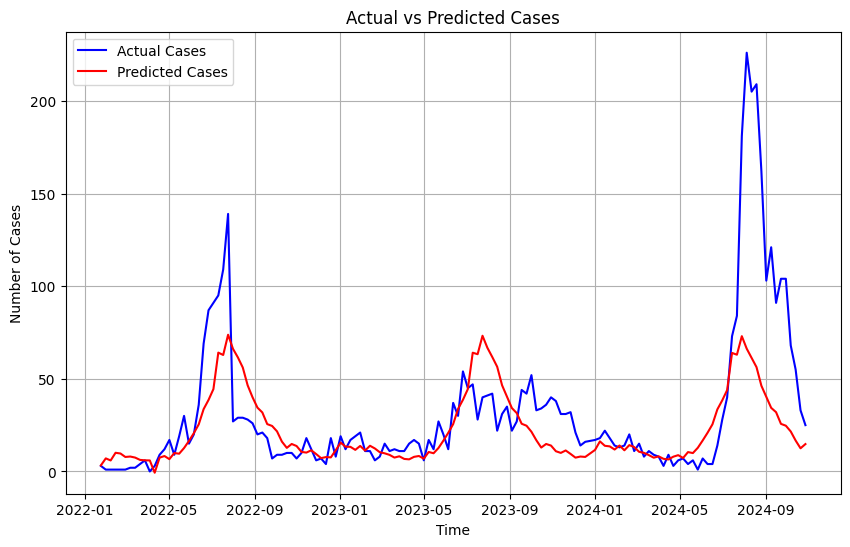
\includegraphics[width=1\textwidth]{line_graph_Sarima}
	\caption{Seasonal ARIMA Prediction Results for Test Set}
	\label{fig:Sarima_result}
\end{figure}

This model incorporates seasonal parameters, which were tuned using grid search to find the best configuration: \textbf{SARIMA(2, 0, 2)(0, 1, 1)[52]}. As with ARIMA, \textbf{400 iterations} were applied to ensure a robust fit. As shown in Figure \ref{fig:Sarima_result}, the SARIMA model demonstrates a notable improvement in performance. Unlike its non-seasonal counterpart, it effectively captures the general trend and aligns more closely with the peaks observed in the actual dengue cases, indicating its ability to model seasonal dynamics.

The model's performance was assessed using regression metrics to evaluate its forecasting capability. The SARIMA model yielded the following error metrics: \begin{itemize} \item \textbf{MSE}: 1109.69 \item \textbf{RMSE}: 33.31 \item \textbf{MAE}: 18.09 \end{itemize} The lower error values, when compared to the ARIMA model, highlight the SARIMA model's superior capability in forecasting dengue cases. Its effectiveness in capturing seasonal patterns contributed to a more accurate representation of the actual cases.

After training the model, the SARIMA model was validated using the same Time Series Cross-Validation strategy employed in the LSTM model. Table \ref{tab:tcsv_sarima} presents the performance metrics for each fold, as well as the average metrics across all folds. The average RMSE and MAE values were close to those obtained during the initial training phase, indicating that the SARIMA model performed consistently across different time segments.

\begin{table}[h!]
	\centering
	\begin{tabular}{|l|c|c|c|}
		\hline
		\textbf{Fold} & \textbf{MSE} & \textbf{RMSE} & \textbf{MAE} \\
		\hline
		1 & 659.68  & 25.68 & 16.00 \\
		2 & 2127.49 & 46.12 & 21.30 \\
		3 & 996.43  & 31.56 & 18.89 \\
		\hline
		\textbf{Average} & \textbf{1261.20} & \textbf{34.45} & \textbf{18.73} \\
		\hline
	\end{tabular}
	\caption{Comparison of SARIMA performance for each fold}
	\label{tab:tcsv_sarima}
\end{table}


\subsection{Kalman Filter Model}

Figure \ref{fig:Kalman_result} shows the comparison between the actual dengue cases and the predicted values on the test set. As illustrated in the plot, the Kalman Filter model demonstrates a moderate ability to follow the general trend of the actual data. While it effectively captures some rising and falling patterns, it still struggles to accurately replicate the sharp peaks and extreme values found in the real case counts. This limitation is particularly noticeable during the large spikes in 2022 and 2024. The model’s performance was evaluated using standard regression metrics. The results are as follows:
\[
\text{MSE} = 1474.82, \quad
\text{RMSE} = 38.40, \quad
\text{MAE} = 22.34
\]
\begin{figure}[H]
	\centering
	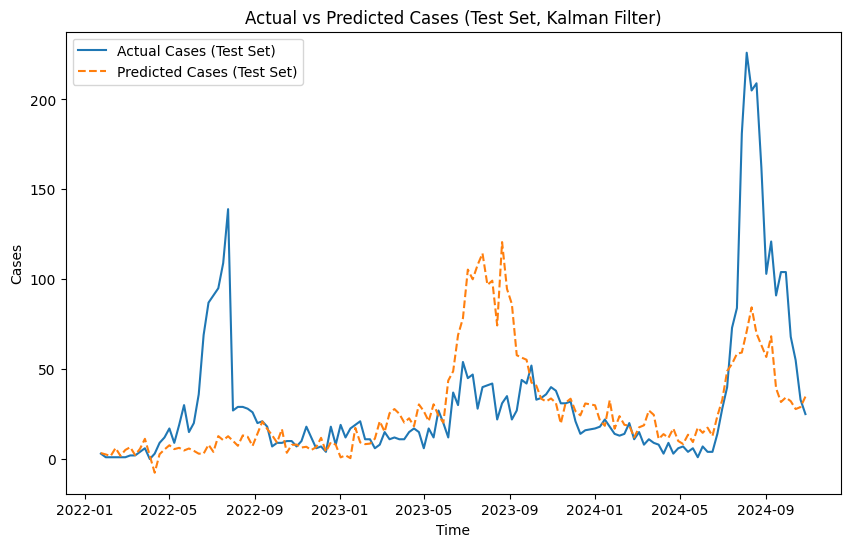
\includegraphics[width=1\textwidth]{line_graph_Kalman}
	\caption{Kalman Filter Prediction Results for Test Set}
	\label{fig:Kalman_result}
\end{figure}

The Kalman Filter was then combined with the LSTM model in order to see improvements in its predictions. Table \ref{tab:tcsv_kflstm} shows the metrics across three folds using the same Time Series Cross Validation Strategy employed in the previous models to see how it performed on different time segments.

\begin{table}[h!]
	\centering
	\begin{tabular}{|l|c|c|c|}
		\hline
		\textbf{Fold} & \textbf{MSE} & \textbf{RMSE} & \textbf{MAE} \\
		\hline
		1 & 113.59  & 10.66 & 6.42 \\
		2 & 752.51 & 27.43 & 12.11 \\
		3 & 1489.95  & 38.60 & 25.13 \\
		\hline
		\textbf{Average} & \textbf{785.35} & \textbf{25.56} & \textbf{14.55} \\
		\hline
	\end{tabular}
	\caption{Comparison of KF-LSTM performance for each fold}
	\label{tab:tcsv_kflstm}
\end{table}

As can be seen in the table above, the performance of the hybrid model demonstrated improvements in all metrics as compared to just using the Kalman Filter alone.

\clearpage
\section{Preliminary System Requirements}
\subsection{Backend Requirements}
\subsubsection{Database Structure Design}
Determining how data flows and how it would be structured is crucial in creating the system as it defines how extendible and flexible it would be for future features and updates. Thus, creating a comprehensive map of data ensures proper normalization that eliminates data redundancy and improves data integrity. Figure \ref{fig:er_diagram} depicts the designed database schema that showcases the relationship between the application's entities. 
\begin{figure}[H]
	\centering
	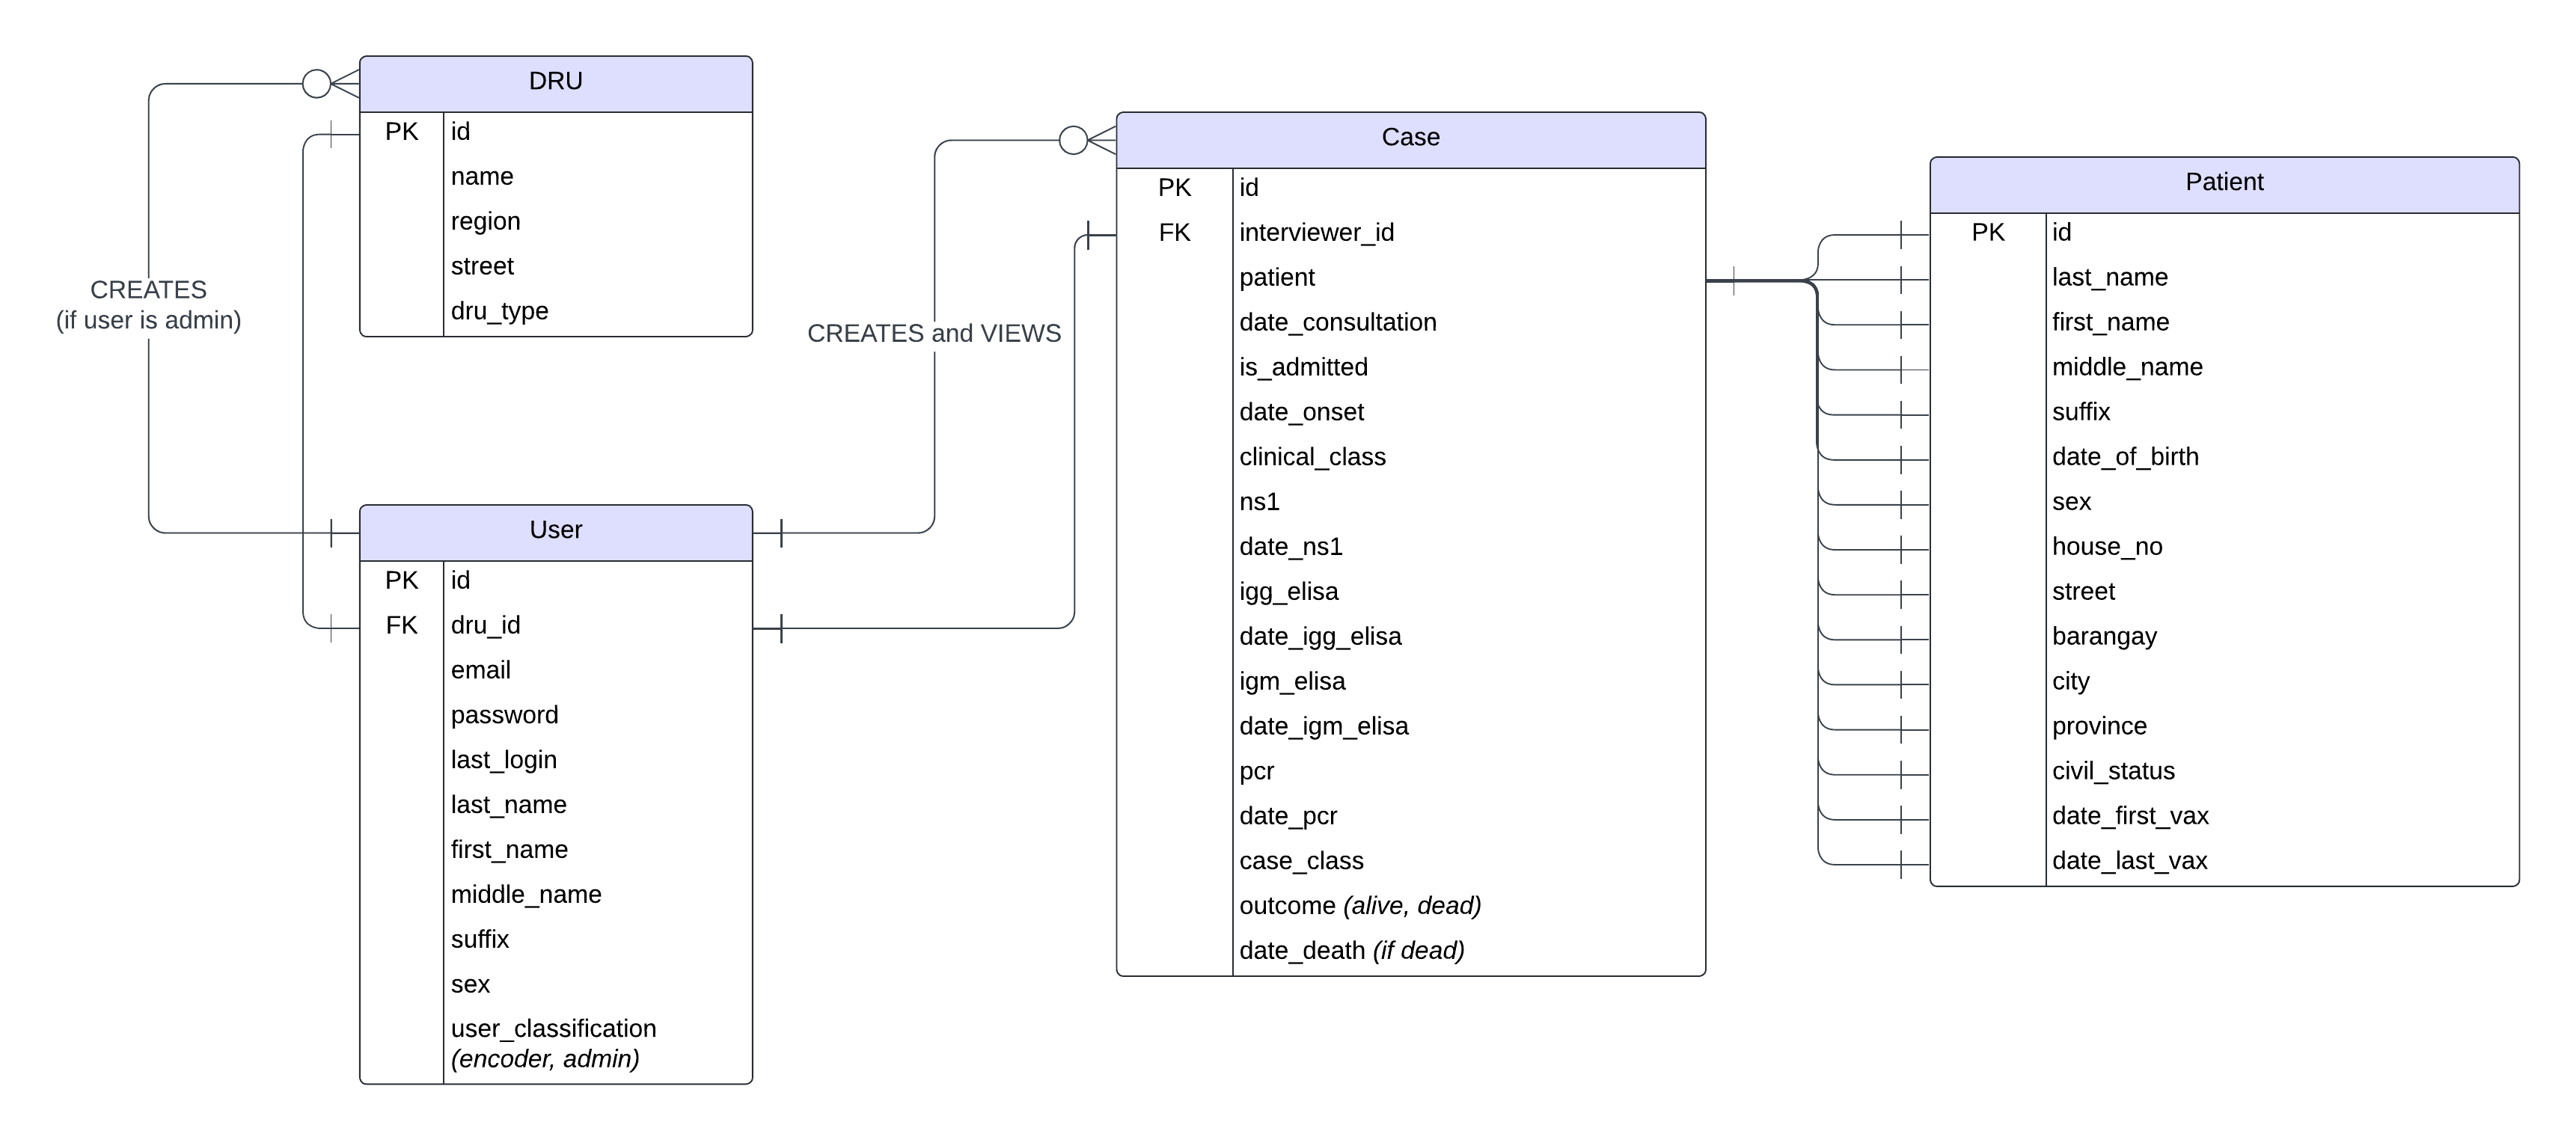
\includegraphics[width=1\textwidth]{er_diagram}
	\caption{Entity-Relationship Database Schema Hybrid Diagram for DengueDash Database Structure}
	\label{fig:er_diagram}
\end{figure}

\subsection{User Interface Requirements}
\subsubsection{Admin Interface}
\begin{figure}[H]
	\centering
	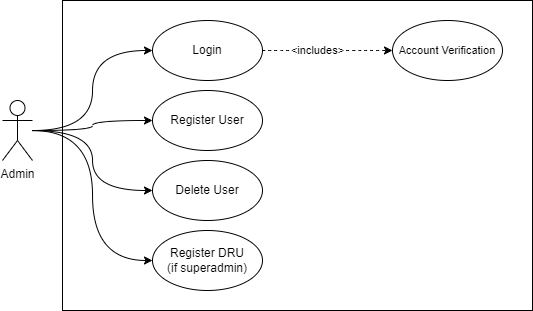
\includegraphics[width=1\textwidth]{admin}
	\caption{Use Case Diagram for Admin}
	\label{fig:admin-use-case}
\end{figure}
Figure \ref{fig:admin-use-case} shows the possible tasks that the admin can do in the application. To protect the integrity of data, only the admins can register and delete accounts. Both account creation and deletion will be done within the application.

\subsubsection{Encoder Interface}
\begin{figure}[H]
	\centering
	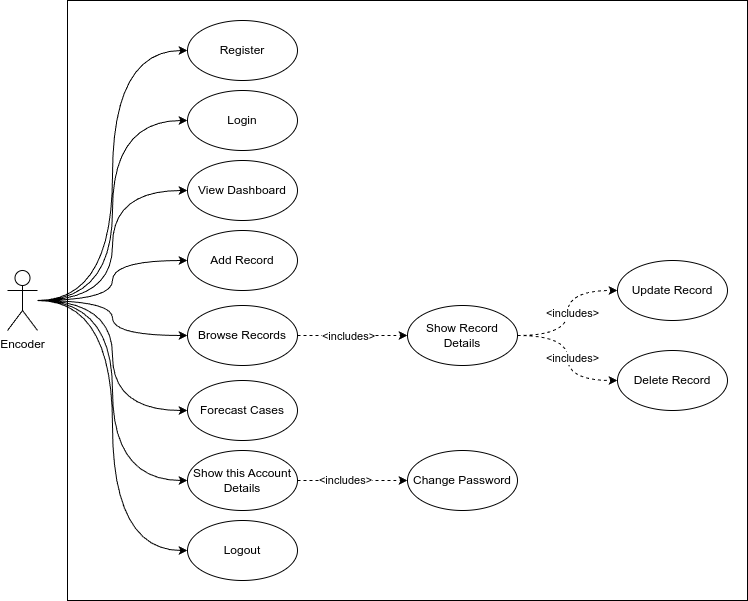
\includegraphics[width=1\textwidth]{encoder}
	\caption{Use Case Diagram for Encoder}
	\label{fig:encoder-use-case}
\end{figure}

Figure \ref{fig:encoder-use-case}, on the other hand, illustrates the use cases for the system's primary users. Since only the admin accounts can register a user, the registration process is not part of it. Instead, the main features, which include reporting and viewing records, are the only permitted actions for this type of user. The said processes can be done in the application by filling out a form with details required for each dengue case. 
As data is entered, it will be consolidated for model training and used for further forecasting of dengue cases.


\subsection{Security and Validation Requirements}
\subsubsection{Password Encryption}
Storing passwords as plain text in the database is a disgrace and a mortal sin in production. It is important to implement precautionary methods such as hashing and salting, followed by encryption with a strong algorithm, to prevent bad actors from using the accounts for malicious transactions. By default, Django generates a unique random salt for each password and encrypts it with Password-Based Key Derivation Function 2 (PBKDF2) with a SHA256 hash function. Utilizing these techniques ensures that in the event of a data breach, cracking these passwords would be time-consuming and useless for the attackers. 

\subsubsection{Authentication}
DengueWatch utilizes JSON Web Tokens (JWT) to authenticate the user. Since the mechanism operates in a stateless manner, tokens are served only after a successful login, eliminating the need for the server to keep a record of the token, which is vulnerable to session hijacking. In addition, these tokens are signed with a secret key, ensuring they have not been tampered with. 

\subsubsection{Data Validation}
Both the backend and frontend should validate the input from the user to preserve data integrity. Thus, Zod is implemented in the latter to help catch invalid inputs from the user. By doing this, the user can only send proper requests to the server which streamlines the total workflow. On the other hand, Django has also a built-in validator that checks the data type and ensures that the input matches the expected format on the server side. These validation processes ensure that only valid and properly formatted data is accepted, which reduces the risk of errors and ensures consistency across the web application. 

\subsection{Testing Process}
\begin{figure}[H]
	\centering
	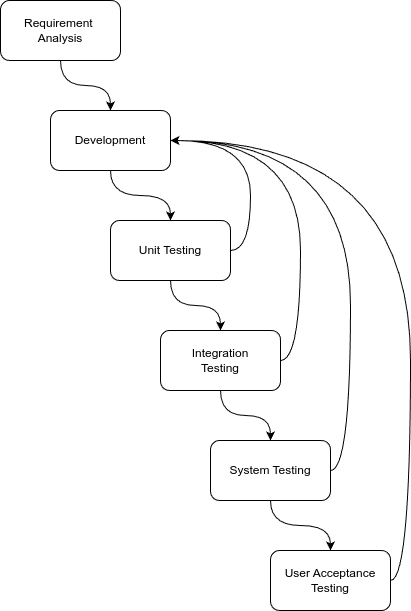
\includegraphics[height=10cm]{testing_process}
	\caption{Testing Process for DengueWatch}
	\label{fig:testing-process}
\end{figure}

As the system requirements and functionalities have been mentioned above, it is important to implement testing to validate the system's performance and efficacy. Since dengue reports include confidential information, anonymized historical dengue reports were used to train the model and create the foundational architecture of the system. By using functional tests, data validation and visualization can be ensured for further continual improvements. Security testing is also important as it is needed to safeguard confidential information when the system is deployed. It includes proper authentication, permission views, and mitigating common injection attacks. Finally, a user acceptance test from the prospected users, in this case, the Iloilo City Epidemiology and Surveillance Unit, is crucial to assess its performance and user experience. It enables the developers to confirm if the system meets the needs of the problem, and once confirmed, it will be deployed and further evaluated to ensure stability and reliability in live operation. 

\section{System Prototype}
\subsection{Guest Interface}
The Guest Interface is intended for all visitors of the web application. It shows the related statistics for dengue cases in a particular area and time. As the system is still in its testing phase, the data converted into charts shown in Figure \ref{fig:guest_dashboard} are generated from Python's Faker library. 
\begin{figure}[H]
	\centering
	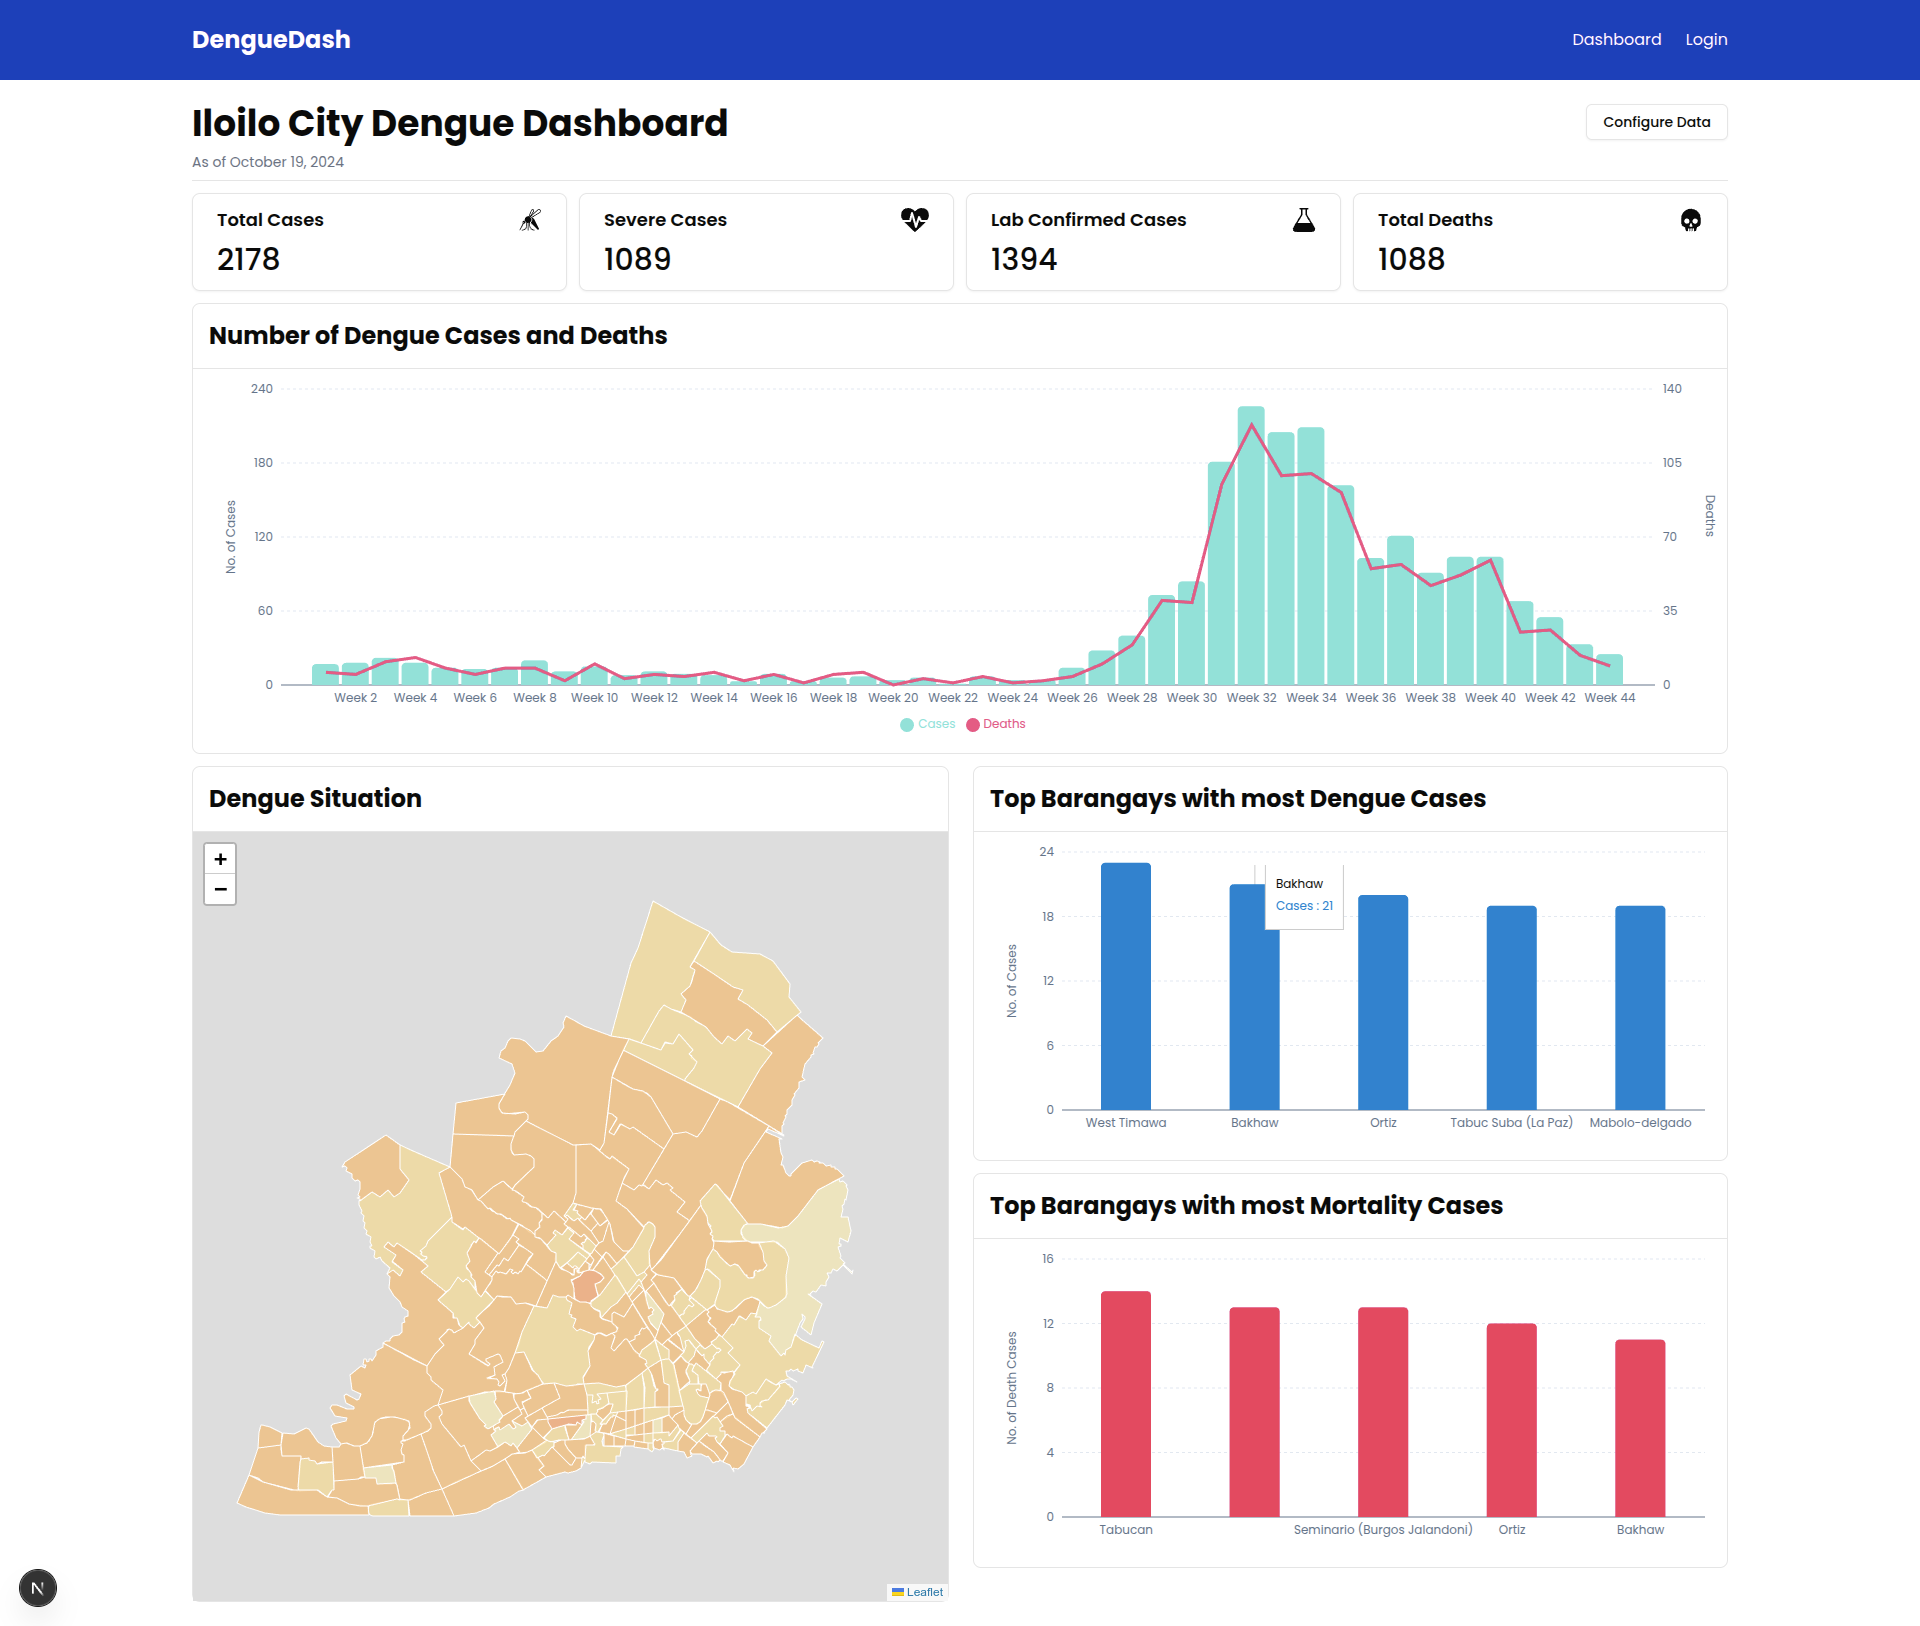
\includegraphics[width=1\textwidth]{guest_dashboard}
	\caption{Dashboard for Guests}
	\label{fig:guest_dashboard}
\end{figure}
\subsection{Personnel Interface}
\subsubsection{User Authentication, and Login}
To protect the data's integrity in production, it has been decided that the registration process will not be visible. Instead, an admin must register a user using a different interface. As of the moment, registering a user is done using API via Postman. In the login process, the system implements HTTP-only cookies that contains the JSON Web Tokens (JWT) to protect against XSS attacks. After proper credentials have been provided, it will redirect to the user's home page.
\begin{figure}[H]
	\centering
	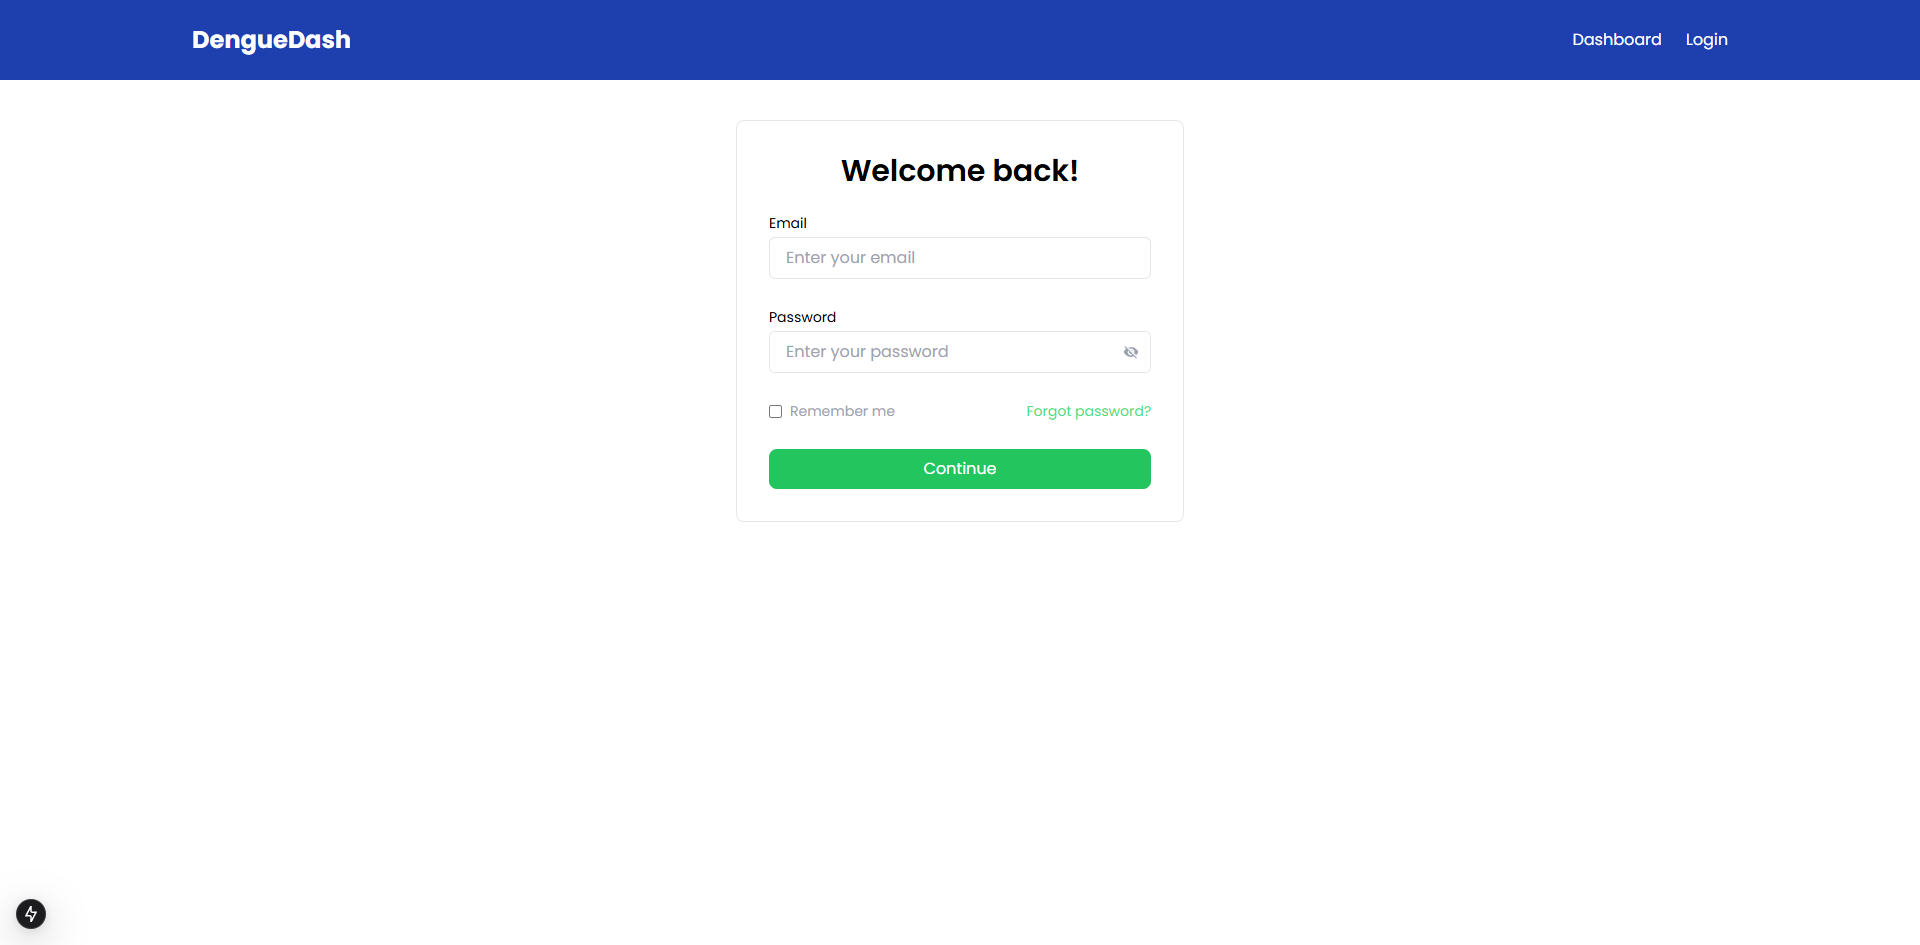
\includegraphics[width=1\textwidth]{login}
	\caption{Login Page for Users}
	\label{fig:login_page}
\end{figure}
\subsubsection{Encoder's View}
Figures \ref{fig:case_report_form_1} and \ref{fig:case_report_form_2} show the digitized counterpart of the form obtained from the Iloilo Provincial Epidemiology and Surveillance Unit. As the system aims to support expandability for future features, some fields were modified to accommodate more detailed input. It is worth noting that all of the included fields adhere to the latest Philippine Integrated Disease and Surveillance Response (PIDSR) Dengue Forms, which the referenced form was based on. By doing this, it is assumed that the targeted users will have a familiarity when deployed on a national scale. On a further note, the case form includes the patient's basic information, dengue vaccination status, consultation details, laboratory results, and the outcome. 
\begin{figure}[H]
	\centering
	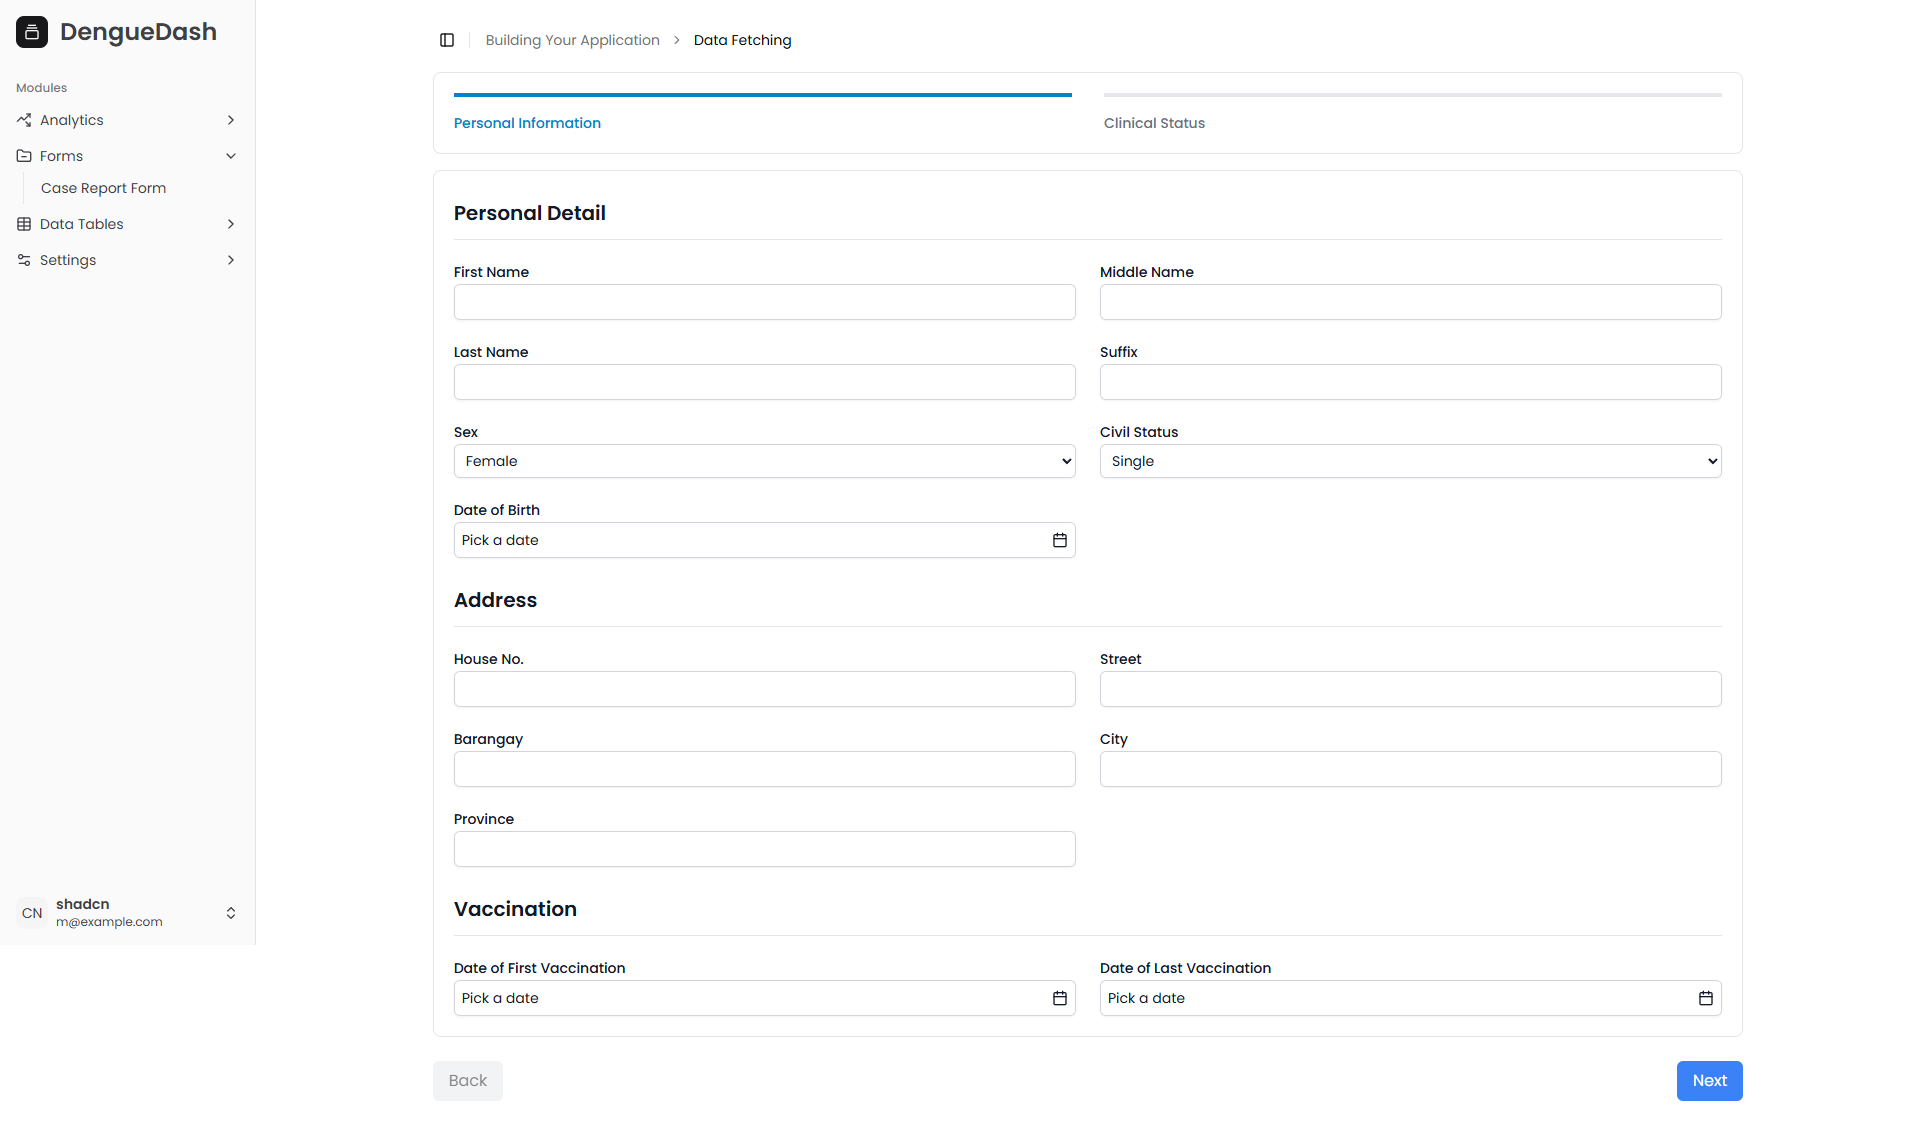
\includegraphics[width=1\textwidth]{case_report_form_1}
	\caption{First Part of Case Report Form}
	\label{fig:case_report_form_1}
\end{figure}
\begin{figure}[H]
	\centering
	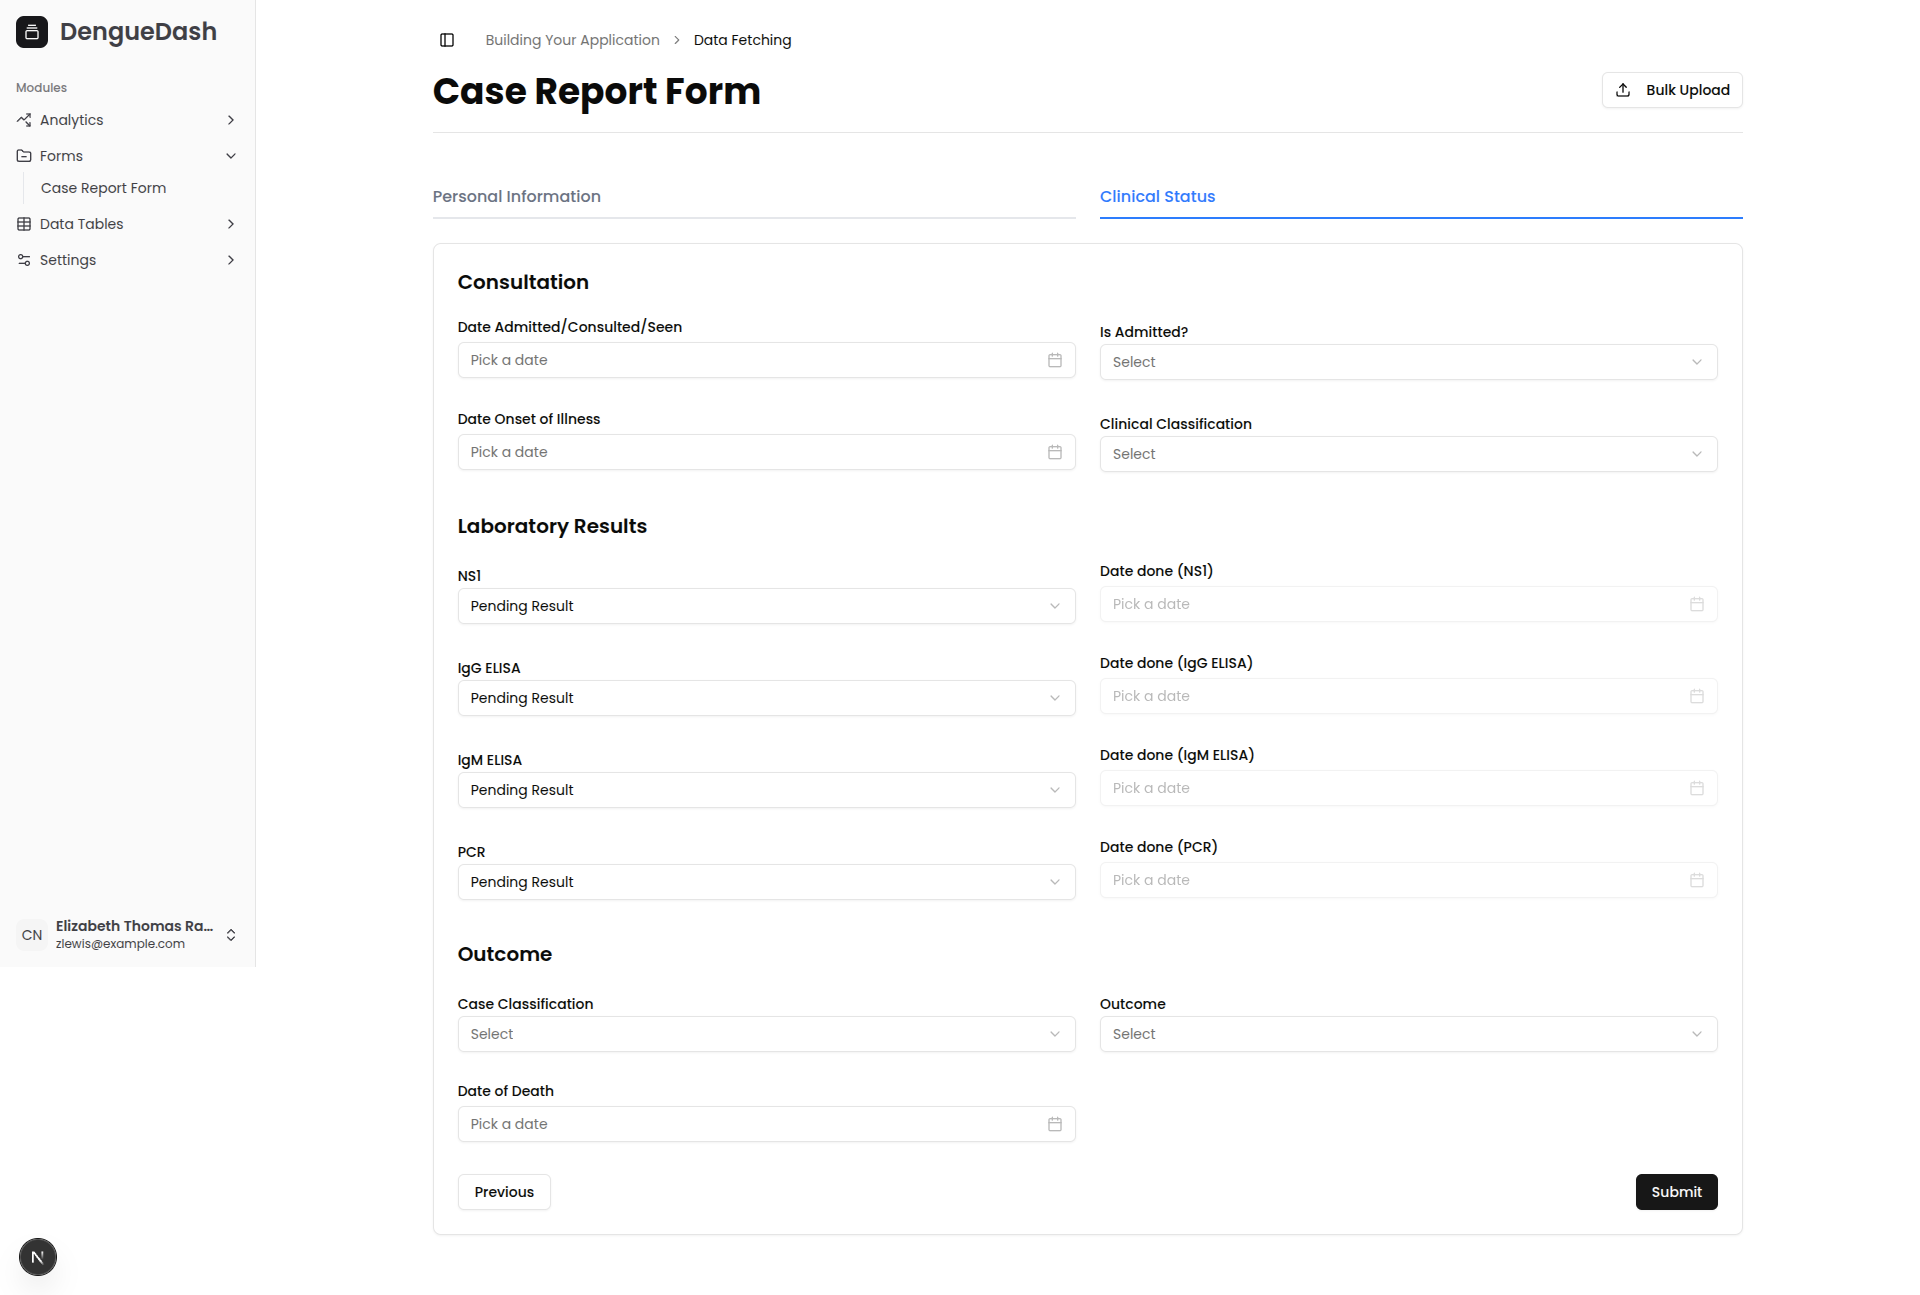
\includegraphics[width=1\textwidth]{case_report_form_2}
	\caption{Second Part of Case Report Form}
	\label{fig:case_report_form_2}
\end{figure}
\clearpage
Once the data generated from the case report form is validated, it will be assigned as a new case and can be accessed through the Dengue Reports page, as shown in Figure \ref{fig:dengue_reports}. The said page displays basic information about the patient related to a specific case, including their name, address, date of consultation, and clinical and case classifications. 
It is also worth noting that it only shows cases the user is permitted to view. For example, in a local Disease Reporting Unit (DRU) setting, the user can only access records that came from the same DRU. On the other hand, in a consolidated surveillance unit such as a regional and provincial quarter, its users can view all the records that came from all the DRUs that report to them. Moving forward, Figure \ref{fig:case_report} shows the detailed case report of the patient on a particular consultation date. 
\begin{figure}[H]
	\centering
	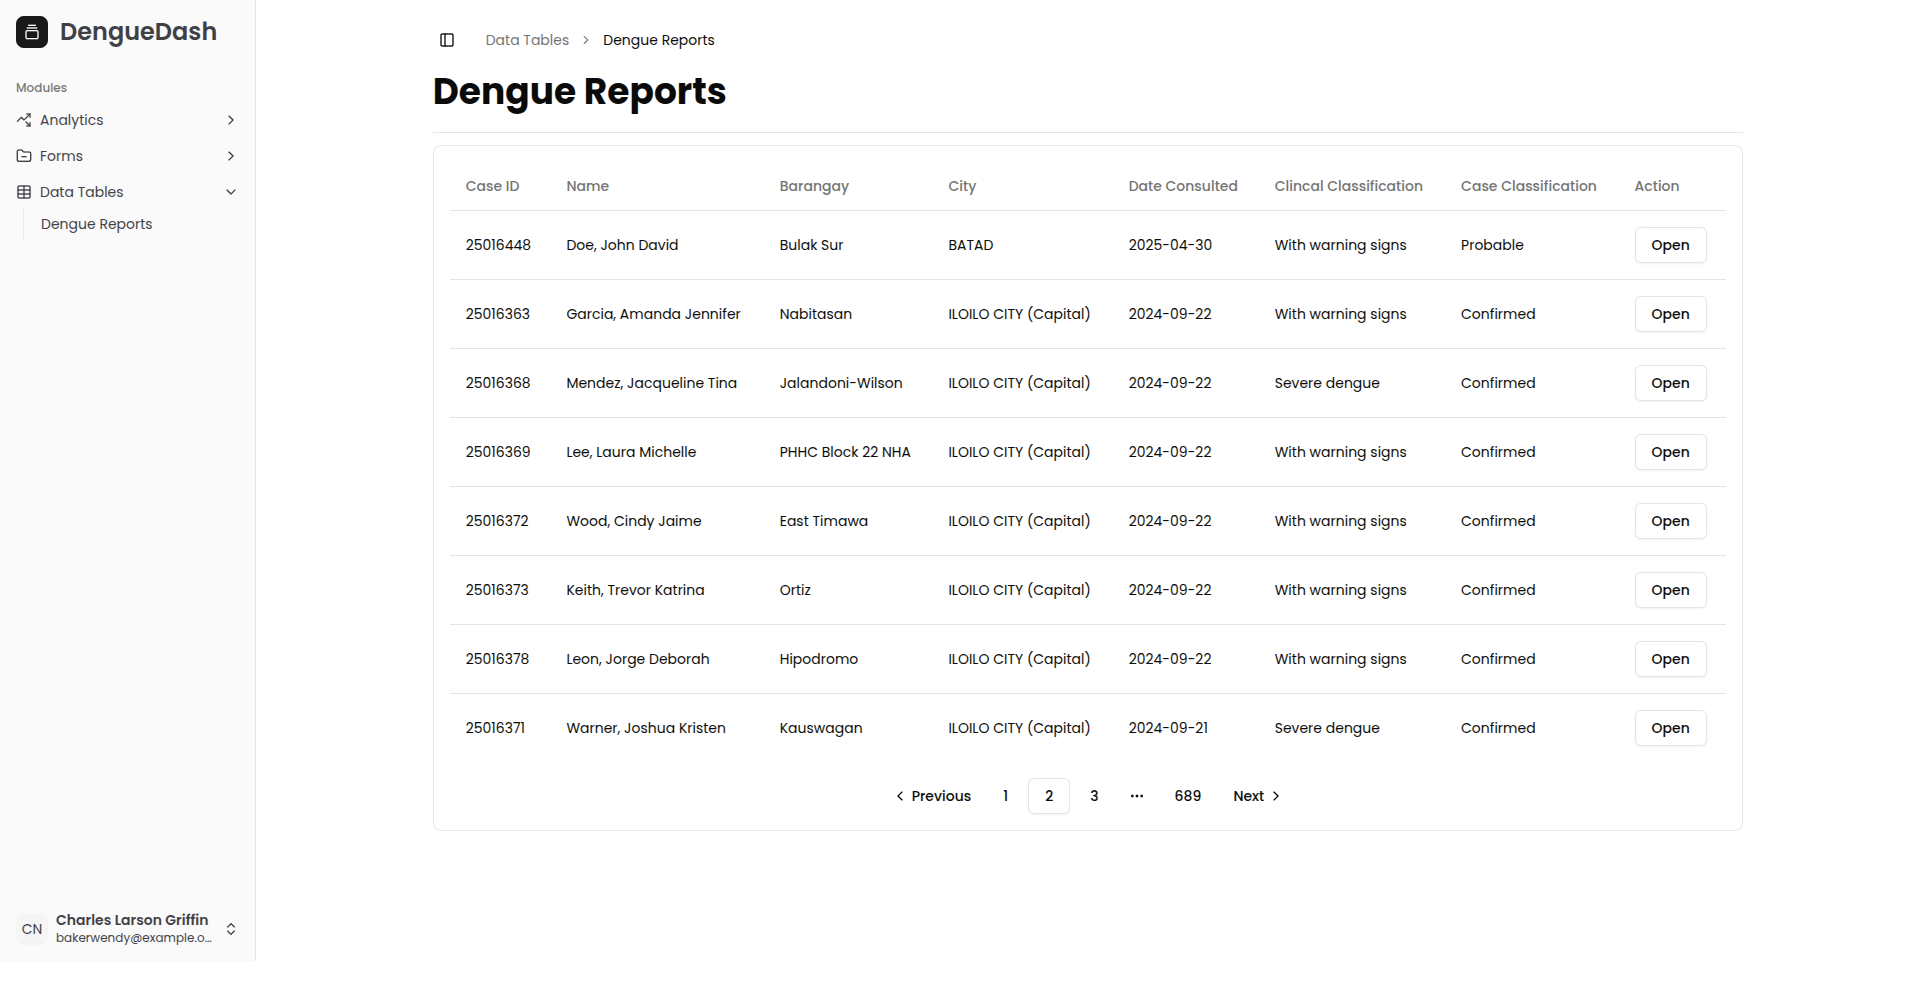
\includegraphics[width=1\textwidth]{dengue_reports}
	\caption{Dengue Reports}
	\label{fig:dengue_reports}
\end{figure}
\begin{figure}[H]
	\centering
	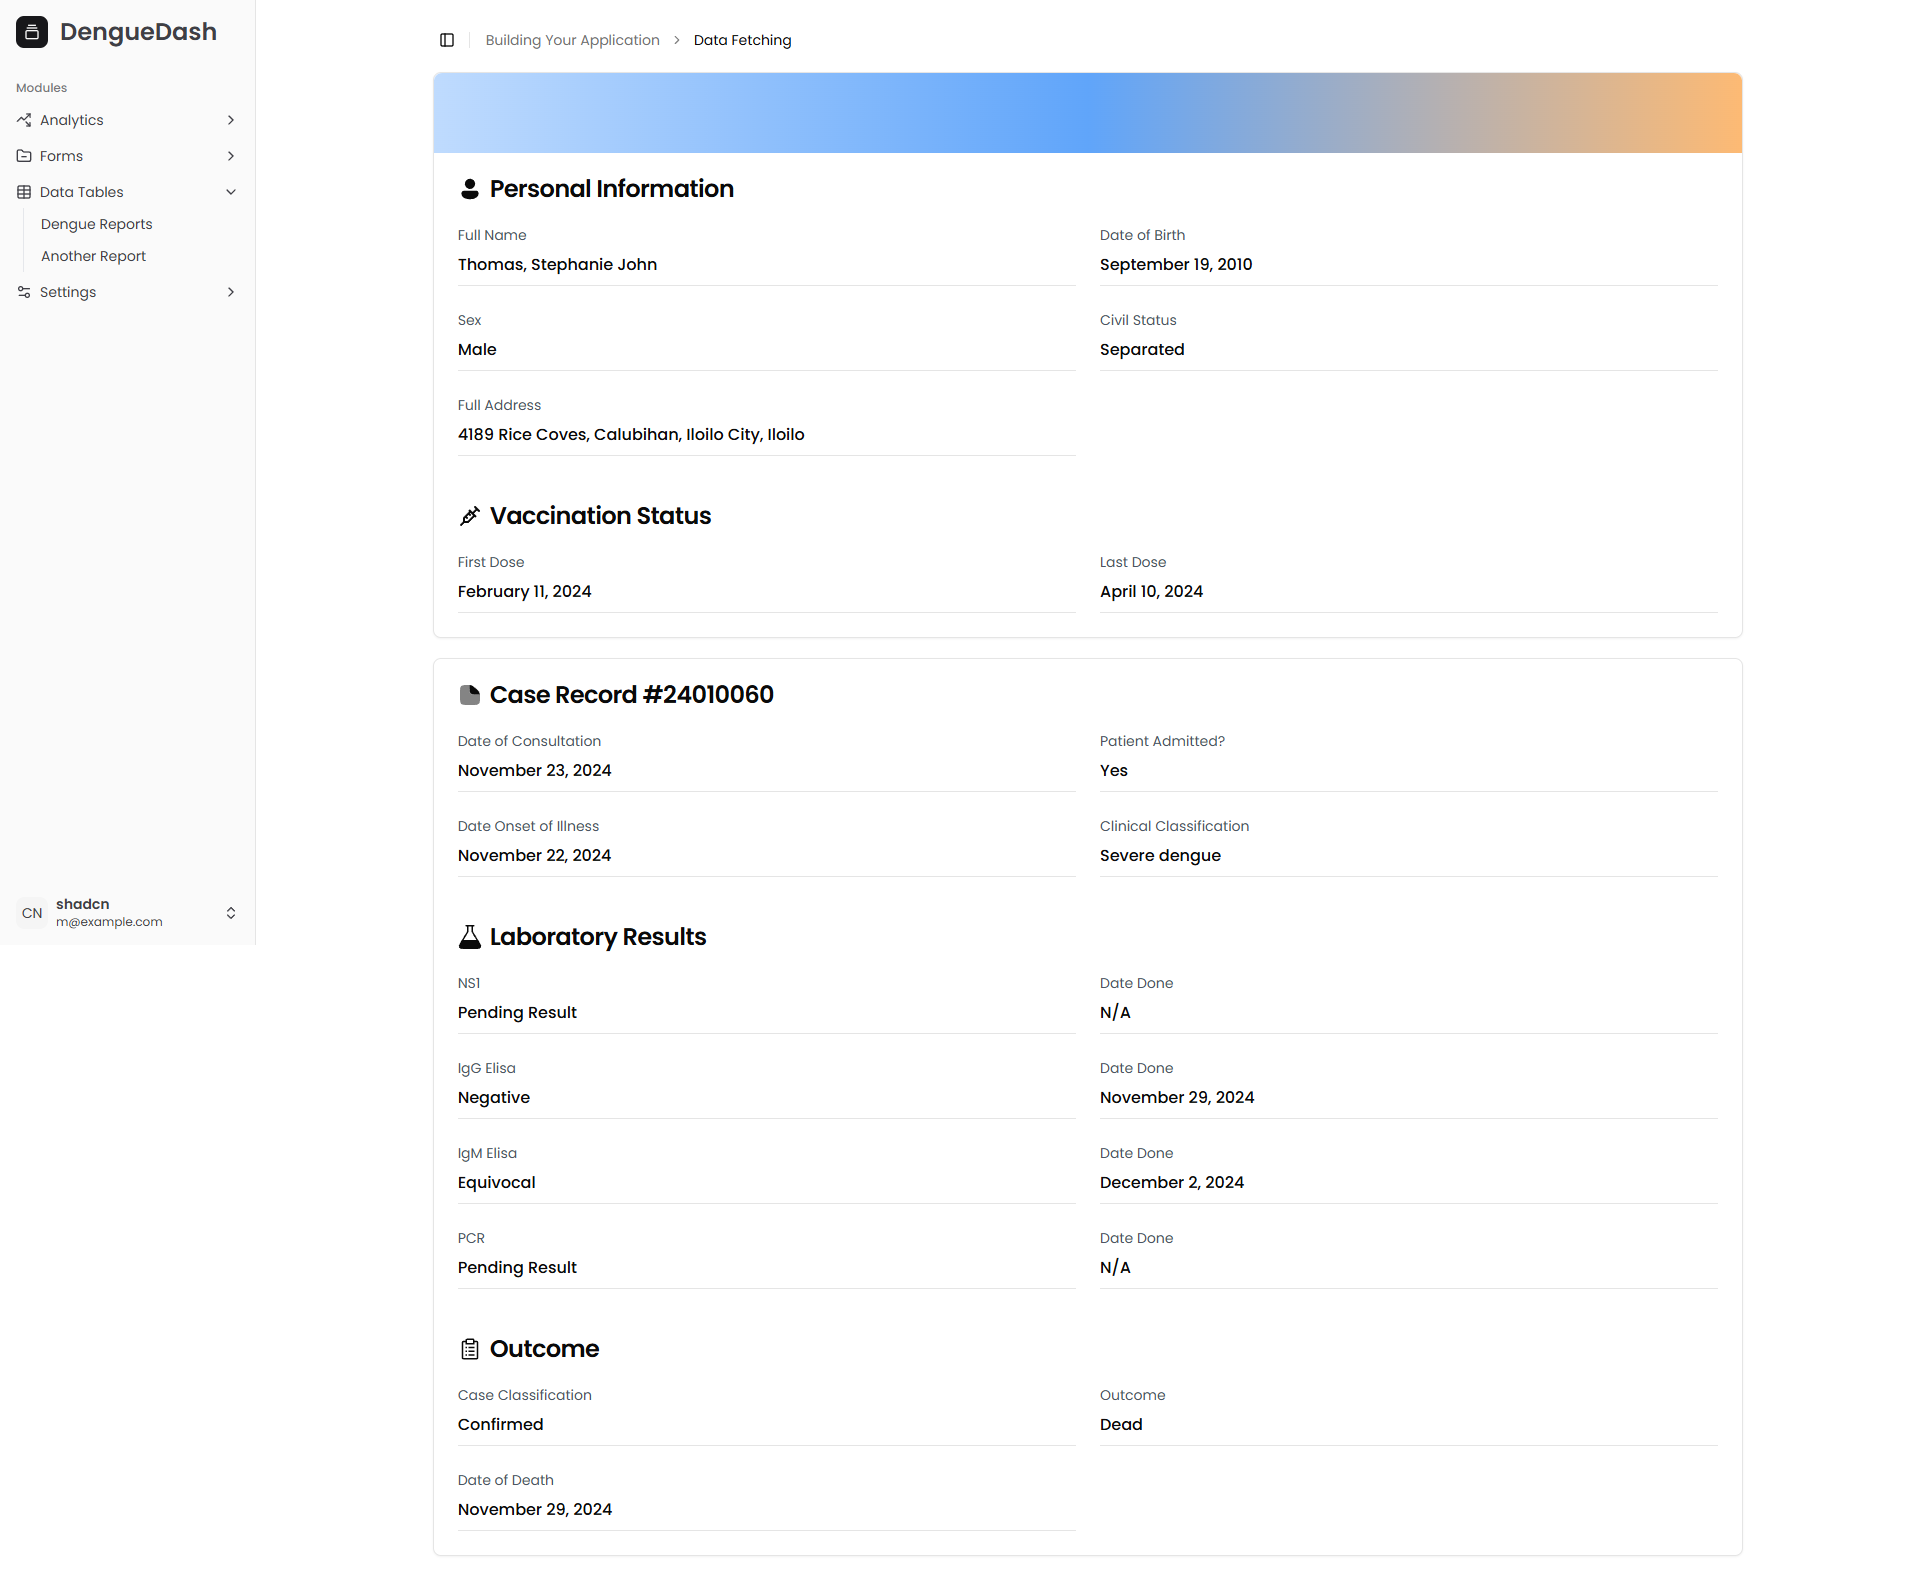
\includegraphics[width=1\textwidth]{case_report}
	\caption{Detailed Case Report}
	\label{fig:case_report}
\end{figure}
